\section{Tuesday, August 30th}
\subsection{Review: LTI (Linear Time-Invariant) Systems}

\subsubsection{Signals are functions}
    \begin{align*}
    &\text{Continuous Time: } x : \mathbb{R} \rightarrow \mathbb{R} 
    \text{ or } x : \mathbb{R} \rightarrow\mathbb{C}
    \\
    &\text{Discrete Time: } x :  \mathbb{Z} \rightarrow \mathbb{R} \text{ or } \mathbb{C}
    \end{align*}
    \[
        x \in X \ \rightarrow \ \boxed{H} \ \rightarrow \  y \in Y
    \]
    where $X$ is the input signal space and $Y$ is the output signal space.
    
    Formally, we say that $y=H(x)$. Note that systems are simply mappings from functions to functions.
    
\subsubsection{Time Invariance}
    \begin{shaded}
    If $\hat x(t)\stackrel{.} = x(t-T)$ then $\hat y(t) \stackrel.= y(t-T)$. In other words, the output must be offset at the same relative amount as the input.
    \end{shaded}
    
\subsubsection{Easy Check for LTI: ZIZO}
    To make sure that linearity is ensured, zero should map to zero. Note that this alone is not enough to prove linearity but it is necessary (e.g. $y(t)=x^2(t)$).

\subsubsection{DT-LTI General IO Derivation}
    \[
        \delta(n) \ \rightarrow \ \boxed{H} \ \rightarrow \  h(n)
    \]
    
    Time-Invariance:
    \[
        \delta(n-k) \ \rightarrow \ \boxed{H} \ \rightarrow \  h(n-k)
    \]
    
    Scaling Property:
    \[
        x(k)\delta(n-k) \ \rightarrow \ \boxed{H} \ \rightarrow \  x(k)h(n-k)
    \]
    
    Additivity:
    \[
        \underbrace{\sum_{k=-\infty}^\infty x(k)\delta(n-k)}_{x(n)} \ \rightarrow \ \boxed{H} \ \rightarrow \  \underbrace{\sum_{k=-\infty}^\infty x(k)h(n-k)}_{y(n)}
    \]
    
    The importance of LTI is that you essentially have invertibility, which allows us to uniquely describe (i.e. characterize) a signal by its impulse response. Note that LTI systems can also be seen as convolutions.

\subsubsection{Commutativity of Convolution}
\begin{shaded}
    \[
        y(n) = (x\star h)(n)=\sum_{k=-\infty}^\infty x(k)h(n-k) = \sum_{\ell = \infty}^{-\infty} x(n - \ell) h(\ell)
        = (h\star x)(n)
    \]
\end{shaded}
    
\subsubsection{Impulse Response of Cascade (Series) Interconnection}
    \[
        x(n)=\delta(n) \ \texttt{->} \ \boxed{f(n)} \ \texttt{->} \ \boxed{g(n)} \ \texttt{->} \  y(n)=(f\star g)(n)
    \]
    
which, via commutativity of convolution, has the same impulse response as the following system:
\[
        x(n)=\delta(n) \ \texttt{->} \ \boxed{g(n)} \ \texttt{->} \ \boxed{f(n)} \ \texttt{->} \  y(n)=(g\star f)(n)
    \]
    % Expect Parallel Interconnection in future lecture xor future exam


\subsection{Simple Moving Average}
\[
    x(n) \ \texttt{->} \ \boxed{h(n)} \ \texttt{->} \  y(n)=\frac1N\sum_{k=0}^{N-1} x(n-k)=\frac{x(n)+\cdots+x(n-N+1)}{N}
\]

Let us compute the impulse response of the system $H$. Letting $x(n)=\delta(n),$ we have \[y(n)=h(n)=\frac{\delta(n)+\delta(n-1)+\cdots+\delta(n-(N-1))}{N},\]
and we depict this signal below:
\begin{figure}[h]
    \centering
    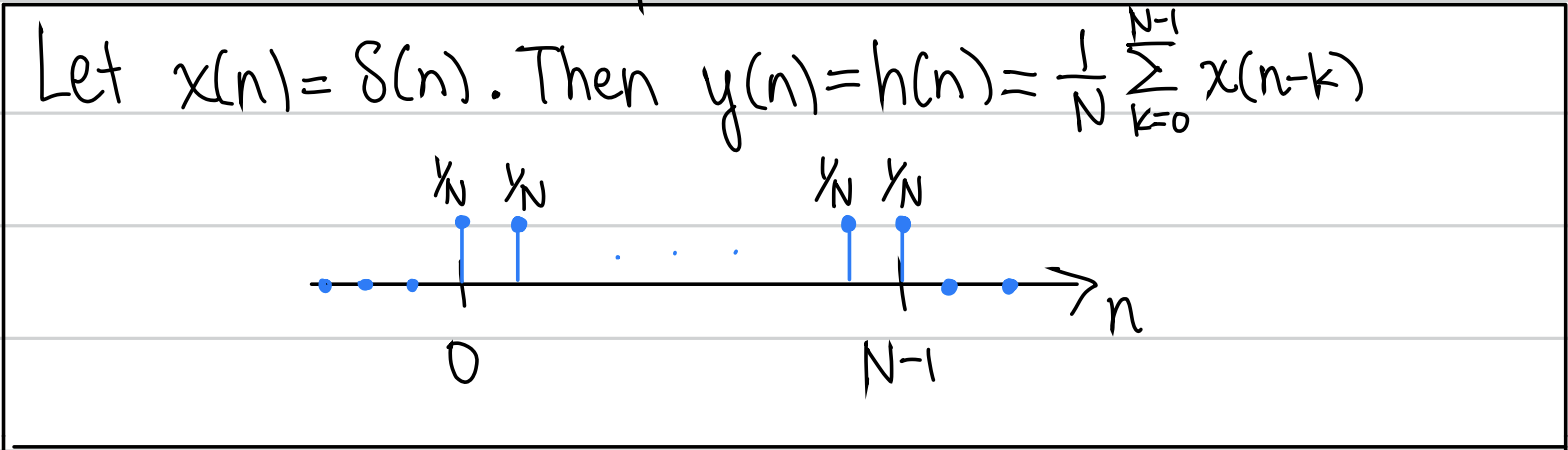
\includegraphics[scale=0.25]{lectures/img/Lec2_SimpleMovingAverage.png}
    \caption{Special thanks to Jonathan Pei for this drawing}
    \label{fig:simple_moving_average}
\end{figure}
